\chapter{\emph{Hamilton-Jacobi} vs \emph{Schrödinger}}

	
\begin{tikzpicture}
	\fill [left color=red!50, right color=teal!50] (0,0) rectangle (6.5,.1);
	\fill [left color=teal!50, right color=blue!50] (6.5,0) rectangle (11.5,.1);
	\end{tikzpicture}



\vspace{10mm}
\begin{adjustwidth}{50pt}{50pt}
\begin{ejemplo}
Vamos a ver la formulación de Hamilton-Jacobi, un ejemplo en el siguiente capítulo y entrar ya en la \emph{Teoría Clásica de Campos} (TCC).

La formulación de Hamilton-Jacobi es la única formulación de la mecánica clásica la que se puede equiparar el concepto de una onda y una partícula y fue lo que usó Schrödinger para formular su famosa ecuación de la mecánica cuántica (MQ).

\end{ejemplo}
\end{adjustwidth}
\vspace{5mm}

\section{Formulación de \emph{Hamilton-Jacobbi}}

\begin{multicols}{2}
\begin{figure}[H]
	\centering
	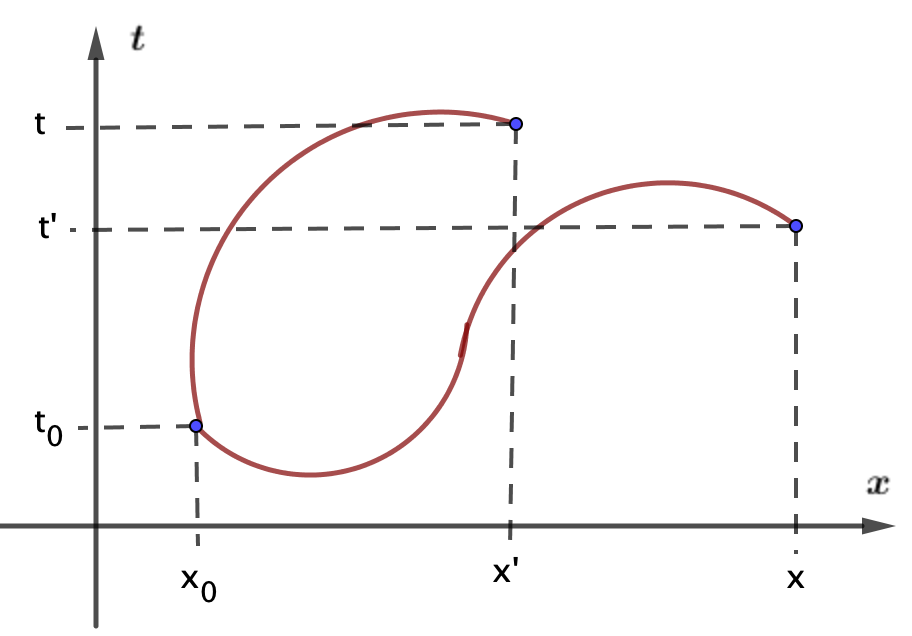
\includegraphics[width=.4\textwidth]{imagenes/img26-01.png}
\end{figure}	
Acción: $\ \displaystyle s[x(t)]=\int_{t_0}^t L\ \dd t =\int_{t_0}^t \left( \dfrac m 2 \dot x^2 - V(x) \right) \dd t$

$(x_0,t_0)\ , \ \ (x,t)\ \ $ son \textbf{puntos fijos}

Dado un campo de fuerzas $V(x)$, la partícula solo tiene una solución que minimiza la acción, la trayectoria real que seguirá.
\end{multicols}

?`Qué ocurriría si moviésemos el punto final $(x,t)$ a otro lugar $(x',t')$ manteniendo el mismo potencial $V(x)$, el mismo campo de fuerzas? Solo habría una nueva curva posible que minimizase la acción que sería aquella por la que se movería la partícula. Si situamos el punto final en un nuevo lugar distinto, habrá una nueva trayectoria real y en cada una de ellas la acción toma un valor determinado. Podríamos considerar la acción $s$ como función del tiempo $t$ y de la posición final $x$, $\ \boldsymbol{ s(x,t) }$. La pregunta es, \textbf{?`cuál es esta función?} Hay dos formas de responder a esta pregunta, A) la de un modo trivial y b) la de suponer que $s(x,t)$ es la solución de una ecuación que aún desconocemos (formulación de Hamilton-Jacobi)

Resumiendo: nos dan un potencial $V(x)$ y un punto inicial fijo $(x_0,t_0)$ y nos preguntan qué vale la acción hasta un punto final $(x,t)$ siguiendo una trayectoria real (acción mínima).

------ \textbf{a) Modo trivial de respuesta a saber quién es} $\boldsymbol{s(x,t)} $

\begin{adjustwidth}{25pt}{5pt}
Suponemos el caso trivial en que $V(x)=0 \ \to \ H=\dfrac {p^2}{2m} $ y las ecuaciones de Hamilton en forma de corchetes de Poisson en este caso son $\dot x =\{x,H\}=\left\{x, \dfrac {p^2}{2m} \right\}=\dfrac {1}{2m}[\ p
\cancelto{1}{\{x,p\}}-\cancelto{1}{\{x,p\}}p ] = \dfrac {1}{2m} (2p)=
\dfrac p m\ $   y también $\ \dot p=\{p,H\}=\left\{p,\dfrac{p^2}{2m} \right\}=0 \ \to \ p=cte \ \to \dot x = \dfrac p m = cte\, ,\  $ por lo que

$\displaystyle s=\int_{t_0}^t \dfrac m 2 \dot x^2 \ \dd t = \dfrac m 2 \dot x^2  \int_{t_0}^t \ \dd t =  \dfrac m 2 \dot x^2  (t-t_0)$

Expresemos $s$ en función del punto final $(x,t)$,

$\dot x =  v =cte \ \to \ v=\dfrac{x-x_0}{t-t_0} \ \Rightarrow \ s=\dfrac m 2 \left( \dfrac{x-x_0}{t-t_0} \right)^2 (t-t_0)=\dfrac m 2 \dfrac{(x-x_0)^2}{t-t_0}$

Y ahora, vamos a hacer algo que hacemos los físicos: indaguemos que es $\displaystyle \pdv{S}{t} \ \text{ y } \ \pdv{S}{x}$

$\triangleright \quad \displaystyle \pdv{S}{t}=-\dfrac m 2 \dfrac{\Delta x^2}{\Delta t^2}=-\dfrac m 2 v^2 = -\dfrac{p^2}{2m} \ \ \textcolor{gris}{(\text{parece} \ -H)} $

$\triangleright \quad \displaystyle \pdv{S}{t} = m\dfrac{\Delta x}{\Delta t} = m v= p $

Nos preguntamos, ?`es esto cierto siempre? Por la definición de acción,

$\displaystyle s=\int_{t_1}^{t_2} L \ \dd t = \int_{t_1}^{t_2} (p\dot x-H) \ \dd t = \int_{t_1}^{t_2} p\dot x \ \dd x - \int_{t_1}^{t_2} H \ \dd t $

Como $\displaystyle \int_a^{a+\varepsilon} f(x) \dd x \approx f(x) \cdot \varepsilon\, , \ $ para $t_2=t_1+\varepsilon$ tendremos

$s\approx p\ \dot x \ \varepsilon \ - \ H \ \varepsilon  \, , \ $
como $\  \dot x = \displaystyle \dv{x}{t} = \dfrac {\Delta x}{\varepsilon } \ \to \ \dot x \ \varepsilon  \approx \Delta x \ $ y, entonces,

$s\approx p\Delta x - H \varepsilon \  $ que confirma lo que pensábamos, $\ \begin{cases} \ \displaystyle \pdv{s}{x}=p \\ \ \displaystyle \pdv{s}{t}=-H \end{cases} \, , \  $  sí se cumple siempre.

$$\subrayado{ \  \textbf{Para } \ \ \ \boldsymbol{ V(x)=0 \ \quad \to \quad \ \displaystyle \pdv{s}{x} \ = \ p  \ \ \wedge \ \ \pdv{s}{t} \ = \ -H } \ } $$

\end{adjustwidth}


------ \textbf{b) formulación de Hamilton-Jacobi}

\begin{adjustwidth}{25pt}{5pt}
Por lo anterior, al sustituir el resultado anterior, $\ \displaystyle p=\pdv{s}{x} \ \  \wedge \ \  	 H=-\pdv{s}{t}\, , \  $ en  el hamiltoniano $\  H=\dfrac{p^2}{2m}+V(x) \ $ tenemos

$\displaystyle -\pdv{s}{t} \ = \ \dfrac 1{2m} \left( \pdv{s}{x} \right)^2 \ + \ V(x) \quad \to \quad \textcolor{red}{\dfrac 1{2m} \left( \pdv{s}{x} \right)^2 \ + \ V(x)} \ + \ \pdv{s}{t}\ = \ 0$

Como $H(q,p)$, podemos escribir la ecuación anterior como $º \displaystyle \textcolor{red}{H\left( q, \pdv{s}{q} \right)} \ + \ \pdv{s}{t} \ = \ 0$

\vspace{5mm} Para más variables, 

\vspace{5mm}

\begin{myalertblock}{Ecuación de hamilton-Jacobi}
\begin{equation}
\boldsymbol{ H\left(q_1,\cdots , q_n, \pdv{s}{q_1}, \cdots , \pdv{s}{q_n} \right) \ + \ \pdv{s}{t} \ = \ 0 }
\end{equation}
\end{myalertblock}

\end{adjustwidth}

\vspace{1cm}
\section{Cómo pudo \emph{Schrödinger} deducir su ecuación}

 
En 1926, Schrödinger había oido que De Broglie, dos años antes, dijo que una partícula de masa $m$ y velocidad $v$ debería tener asociada una onda de longitud $\lambda$ de modo que $\lambda$ y $p$ estuviesen relacionadas.

Schrödinger conocía la formulación de Hamilton-Jacobi y sabía que era útil para describir fenómenos ondulatorios.

\begin{multicols}{2}
Onda: $\ y=A\cos(Kx-\omega t)$

Para operar es mejor considerar $\ y=Ae^{i(Kx-\omega t)}$ y, al acabar, tomar la parte real.

Schrödinger pensó en una onda de ecuación $\psi(t,x)=e^{i\ \text{fase}}$

La acción cumple que $\ \displaystyle \pdv{s}{x}=p \ \wedge \ \pdv{s}{t}=-H=-E$

\begin{figure}[H]
	\centering
	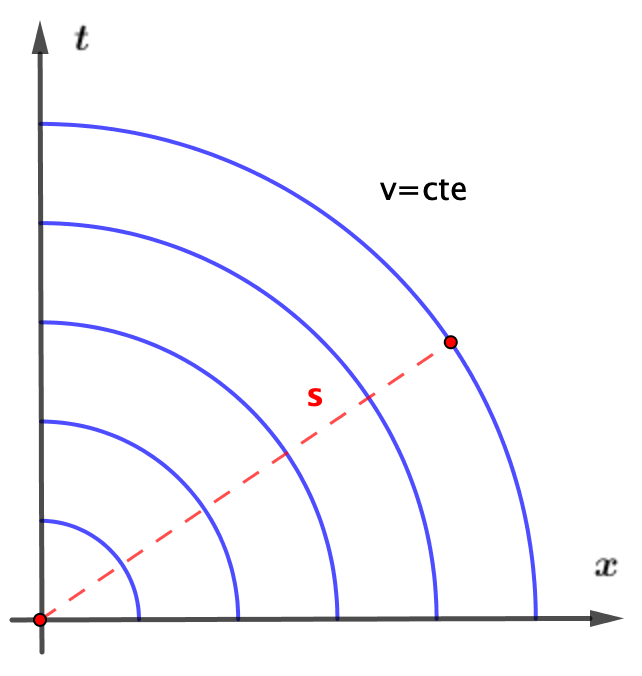
\includegraphics[width=.3\textwidth]{imagenes/img26-02.png}
\end{figure}	
\end{multicols}

Con $v=cte \ \to \ p=cte \ \to \ E=cte \ \Rightarrow \ S=-Et+px\, ,  \ $ que será la fase de nuestra onda. Pero la fase debe ser adimensional y esto tiene dimensiones de \emph{energía $\cdot$ tiempo} y, casualmente, $\ \hbar \ $ tiene estas mismas dimensiones, entonces $\left[ \dfrac s \hbar \right] = 1 \, , \ $ adimensional, y es lo que tomaremos como fase.

$$ \psi(t,x) \ = \ e^{i \left( -\dfrac E \hbar \ t \ + \ \dfrac p \hbar \ x \right)} \ = \ e^{i \dfrac {s(t,x)}{\hbar}}$$

Este será nuestro prototipo de onda que no sabemos a que responde.

Volvemos a usar el truco de los físicos, derivemos a ver qué ocurre \textcolor{gris}{(es lo normal a la hora de buscar ecuaciones)}

$\triangleright \qquad \displaystyle \pdv{\psi}{t}=ºpsi i \left( -\dfrac E \hbar \right) =-i \psi \dfrac 1 \hbar E=-i \psi \dfrac 1 \hbar \dfrac {\textcolor{blue}{\boldsymbol{ p^2 }} }{2m}$

$\triangleright \qquad \displaystyle \pdv{\psi}{x}=\psi i \left( \dfrac p \hbar \right) \ \to \  
\displaystyle \pdv[2]{\psi}{x}=\psi i^2 \left( \dfrac p \hbar \right)^2 =  - \psi \dfrac 1{\hbar^2} \textcolor{blue}{\boldsymbol{ p^2}}$


Despejando $\qquad \displaystyle \textcolor{blue}{\boldsymbol{p^2}}=\dfrac{2m\hbar}{-i\psi} \pdv{\psi}{t} \qquad \qquad \qquad \textcolor{blue}{\boldsymbol{p^2}} = \dfrac{\hbar^2}{-\psi} \pdv[2]{\psi}{x} \qquad $ e igualando,

\vspace{5mm}
\begin{myblock}{Ecuación se Schrödinger para $V(x)=0$}
	
\begin{equation}
\boldsymbol{
 -\dfrac{\hbar^2}{2m} \ \pdv[2]{\psi}{x} \ = \ i\ \hbar \ \pdv{\psi}{t}
 }
\end{equation}

\end{myblock}

\vspace{5mm}
Si hubiésemos considerado $V(x) \neq 0$, hubiésemos obtenido

\vspace{5mm}
\begin{myblock}{Ecuación se Schrödinger}
	
\begin{equation}
\boldsymbol{
i\ \hbar \ \pdv{\psi}{t} \ = \  -\dfrac{\hbar^2}{2m} \ \pdv[2]{\psi}{x}  \ + \ V(x) \ \psi
 }
\end{equation}

\end{myblock}

















